\chapter{Transport in Small MOSFETs}
\section{Ballistic Transport}
In a very small channel length MOSFET, the electron can travel through the device without any scatterings, which is called the ballistic transport. If the drain of MOSFET is biased at a high voltage $V_{DS}$, the band diagram would look like Fig. 5.1. The electron at the top of channel is the most important contribution to the current. This approach is called the {\bf top-of-the-barrier model}.
\begin{figure}[tbp]
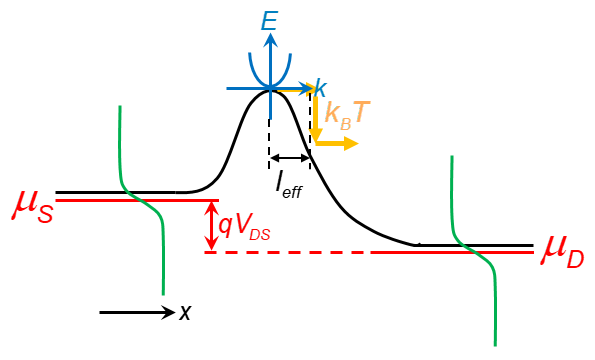
\includegraphics[width=0.6\textwidth]{figures/Fig5_1}
\centering
\caption{\small Band diagram of a small MOSFET.}
\end{figure}
In general, the current at the top-of-barrier can be expressed as \begin{equation}
    I = (-e)W(n_{S}^{+}v_{inj}^{+}-n_{S}^{-}v_{inj}^{-})
\end{equation} where the $n_{S}^{+(-)}$ are the numbers of electrons that injects to the $+x$- and $-x$-directions, the $v_{inj}^{+(-)}$ are the injection velocities to the $+x$- and $-x$-directions, and $W$ is the device width. The electron concentration $Q_{S}$ at the top-of-barrier is related to the gate voltage $V_{G}$. \begin{equation}
    Q_{S} = C(V_{G}-V_{REF})
\end{equation} where $C$ is the gate capacitance and $V_{REF}$ is the reference voltage that determines at which $V_{G}$ there is no electron in the channel. Since the Fermi level of drain side is far away from the conduction band edge in the channel, the electron injection from the drain can be neglected \begin{equation}
    I \approx (-e)Wn_{S}^{+}v_{inj}^{+}
\end{equation} and \begin{equation}
    n_{S} = n_{S}^{+} + n_{S}^{-} \approx n_{S}^{+} = \frac{C(V_{G}-V_{REF})}{-e}
\end{equation} Thus, \begin{equation}
    I = WC(V_{G}-V_{REF})v_{inj}^{+}
\end{equation} which describes the {\bf ballistic transport} in MOSFET.
\section{Transport with Scatterings (Quasi-Ballistic Transport)}
Since there are scatterings in the channel, there are some back-scattered electron $n_{S}^{-}$ but they are only small portion of the $+x$-direction injection \begin{equation}
    n_{S}^{-} = rn_{S}^{+}
\end{equation} where $r$ is the reflection coefficient. Note that the $n_{S}^{+(-)}$ are coming from the source side injection instead of the drain side as mentioned earlier. Since after scattering the electron only loses energy less or equal to $k_{B}T$, the back-scattered electron also has a velocity $v_{inj}^{-}$ close to the $v_{inj}^{+}$. Hence, the current becomes \begin{align}
    I& = (-e)Wn_{S}^{+}v_{inj}^{+}(1-r),\quad n_{S} = n_{S}^{+} + n_{S}^{-} = n_{S}^{+}(1+r)\nonumber\\
    & = (-e)n_{S}Wv_{inj}^{+}\frac{1-r}{1+r}W\nonumber\\
    & = WC(V_{G}-V_{REF})v_{inj}^{+}\frac{1-r}{1+r}
\end{align} Recall the transmission and reflection coefficients \begin{equation}
    T = \frac{\lambda}{\lambda + L}, \quad r = 1 - T = \frac{L}{\lambda + L}
\end{equation} The device length $L$ should be replaced by $l_{eff}$ as defined in Fig. 5.1 because the detailed simulations show that if the electron travels more than 1 to 2 times $\frac{k_{B}T}{q}$ down a potential drop, it is unlikely to re-emerge even if it does backscatter\footnote{M. Lundstrom, Fundamentals of Carrier Transport, 2nd edition, p. 344.}. Thus, the current becomes \begin{equation}
    I = WC(V_{G}-V_{REF})v_{inj}^{+}\frac{1}{1+2\frac{l_{eff}}{\lambda}}
\end{equation} Near equilibrium, the Einstein-Smoluchowski equation states that \begin{equation}
    \frac{2D}{\lambda} = v_{T},\quad \frac{D}{\mu} = \frac{k_{B}T}{e} 
\end{equation} where $D$ is the diffusion coefficient,$\mu$ is the low-field mobility, and $v_{T}$ is the thermal velocity. The electric field $E$ near the top-of-barrier can be estimated using \begin{equation}
    E_{top} = \frac{\frac{k_{B}T}{e}}{l_{eff}}\quad\Leftrightarrow\quad l_{eff} = \frac{k_{B}T}{eE_{top}}
\end{equation} Hence, \begin{align}
    I& = WC(V_{G}-V_{REF})v_{inj}^{+}\frac{1}{1+\frac{2k_{B}T/e}{\lambda E_{top}}},\quad \frac{2k_{B}T/e}{\lambda E_{top}}=\frac{2D}{\lambda}\frac{1}{\mu E_{top}} = \frac{v_{T}}{\mu E_{top}}\nonumber\\
    & = WC(V_{G}-V_{REF})\frac{v_{inj}^{+}}{1+\frac{v_{T}}{\mu E_{top}}}
\end{align} When the device is very long, $E_{top}$ is very small and thus $v_{T}\gg\mu E_{top}$. Thus, the current is back to the standard MOSFET current equation \begin{align}
    I& \approx W\mu C(V_{G}-V_{REF})\left(\frac{v_{inj}^{+}}{v_{T}}\right)E_{top}\nonumber\\
    & \approx \frac{W}{L}\mu C(V_{G}-V_{REF})\left(\frac{v_{inj}^{+}}{v_{T}}\right)V_{DS},\quad V_{DS} \approx \frac{E_{top}}{L}
\end{align}
\section{Generalized Ballistic Transport in One Dimension}
The concept of the injection velocity has been introduced in the previous sections. The injection velocity can be interpreted as the average velocity that the electrons travel from the top-of-the-barrier. \begin{equation}
    \big<v\big> = \frac{\sum_{k_{x}>0}{fv_{k_{x}}}}{\sum_{k_{x}>0}{f}}
\end{equation} where we define\footnote{The pre-factor is $\frac{1}{2\pi}$ instead of $\frac{L}{2\pi}$ because we are calculating the electron "density."} \begin{align}
    Z& \equiv \sum_{k_{x}>0}{fv_{k_{x}}} = \frac{1}{2\pi}\int_{0}^{\infty}dk_{x}\frac{1}{1+e^{\frac{E-\mu}{k_{B}T}}}\frac{\hbar k_{x}}{m^{*}},\quad E=E_{C}+\frac{\hbar^{2}k_{x}^{2}}{2m^{*}},\quad \frac{\mu-E_{C}}{k_{B}T}\equiv \eta \nonumber\\
    & = \frac{1}{2\pi}\frac{\hbar}{m^{*}}\int_{0}^{\infty}k_{x}dk_{x}\frac{1}{1+e^{\frac{\hbar^{2}k_{x}^{2}}{2m^{*}k_{B}T}}e^{-\eta}},\quad \frac{\hbar^{2}k_{x}^{2}}{2m^{*}k_{B}T}\equiv x\nonumber\\
    & = \frac{1}{2\pi}\frac{\hbar}{m^{*}}\frac{m^{*}k_{B}T}{\hbar^{2}}\int_{0}^{\infty}dx\frac{1}{1+e^{x-\eta}}\nonumber\\
    & = \frac{k_{B}T}{2\pi\hbar}\Gamma(1)\Im_{0}(\eta),\quad \Im_{p}(\eta) = \frac{1}{\Gamma(p+1)}\int_{0}^{\infty}dx\frac{x^{p}}{1+e^{x-\eta}}
\end{align} and \begin{align}
    Z_{2}& \equiv \sum_{k_{x}>0}{f} = \frac{1}{2\pi}\int_{0}^{\infty}dk_{x}\frac{1}{1+e^{\frac{\hbar^{2}k_{x}^{2}}{2m^{*}k_{B}T}}e^{-\eta}}\nonumber\\
    & = \frac{1}{2\pi}\frac{m^{*}k_{B}T}{\hbar^{2}}\frac{\hbar}{\sqrt{2m^{*}k_{B}T}}\int_{0}^{\infty}dx\frac{x^{-1/2}}{1+e^{x-\eta}}\nonumber\\
    & = \frac{1}{2\pi\hbar}\frac{\sqrt{m^{*}k_{B}T}}{\sqrt{2}}\sqrt{\pi}\Im_{-1/2}(\eta)
\end{align} Therefore, the average velocity is \begin{equation}
    \big<v\big> = \sqrt{\frac{2k_{B}T}{\pi m^{*}}}\frac{\Im_{0}(\eta)}{\Im_{-1/2}(\eta)}
\end{equation} where \begin{equation}
    \sqrt{\frac{2k_{B}T}{\pi m^{*}}} \equiv v_{T}
\end{equation} is the thermal velocity. If the semiconductor is non-degenerate doped ($\frac{E_{C}-\mu}{k_{B}T}\geq 3k_{B}T\Leftrightarrow \eta\geq -3$), the Fermi integral can be approximated by \begin{equation}
    \int_{0}^{\infty}dx\frac{1}{1+e^{x-\eta}}\approx\int_{0}^{\infty}dxe^{-x}e^{\eta} = e^{\eta}
\end{equation} Thus, \begin{equation}
    Z = \frac{k_{B}T}{2\pi\hbar}e^{\eta}
\end{equation} and \begin{equation}
    Z_{2} = \frac{\sqrt{m^{*}k_{B}T}}{2\pi\hbar}\frac{1}{\sqrt{2}}e^{\eta}\sqrt{\pi}
\end{equation} where \begin{equation}
    \int_{0}^{\infty}x^{-1/2}e^{-x} = \Gamma\left(\frac{1}{2}\right) = \sqrt{\pi}
\end{equation} For non-degenerate semiconductor, the average velocity is \begin{equation}
    \big<v\big> = \sqrt{\frac{2k_{B}T}{\pi m^{*}}} \approx 1.2\times10^7 \quad\text{cm/sec for silicon}
\end{equation} The ballistic current at the top-of-the barrier considering the injection from the source and drain is\footnote{In Section 5.1 and 5.2, the injection from the drain is ignored.} \begin{equation}
    I = W(-e)\underbrace{2}_{\text{spin}}\left(\sum_{k_{x}>0,k_{y}}{fv_{k_{x}}}-\sum_{k_{x}<0,k_{y}}{fv_{k_{x}}}\right)
\end{equation} where the first term is coming from the source side while the second term comes from the drain side \begin{align}
    F^{+}& \equiv \sum_{k_{x}>0,k_{y}}{fv_{k_{x}}} = \frac{1}{4\pi^{2}}\int_{-\infty}^{\infty}dk_{y}\int_{0}^{\infty}dk_{x}\frac{1}{1+e^{\frac{E-\mu_{S}}{k_{B}T}}}\frac{\hbar k_{x}}{m^{*}},\quad E=E_{C}+\frac{\hbar^{2}}{2m^{*}}\underbrace{\left(k_{x}^{2}+k_{y}^{2}\right)}_{k^{2}}\nonumber\\
    & = \frac{1}{4\pi^{2}}\int_{0}^{\pi}d\theta\int_{0}^{\infty}kdk\frac{1}{1+e^{\frac{\hbar^{2}k^{2}}{2m^{*}k_{B}T}}e^{-\eta_{S}}}\frac{\hbar}{m^{*}}k\sin{\theta}\nonumber\\
    & = \frac{1}{4\pi^{2}}\frac{\hbar}{m^{*}}2\frac{m^{*}k_{B}T}{\hbar^{2}}\frac{\sqrt{2m^{*}k_{B}T}}{\hbar}\underbrace{\int_{0}^{\infty}dx\frac{x^{1/2}}{1+e^{x-\eta_{S}}}}_{=e^{\eta_{S}}\Gamma(\frac{3}{2})\approx e^{\eta_{S}}\frac{\sqrt{\pi}}{2},\quad\text{if non-degenerate}}\nonumber\\
    & \approx \underbrace{\frac{1}{2}}_{\text{moving in $+x$ direction}}\underbrace{\left(\frac{m^{*}k_{B}T}{2\pi\hbar^{2}}\right)}_{\text{number of electrons within $k_{B}T$}}\underbrace{\left(\sqrt{\frac{2k_{B}T}{\pi m^{*}}}\right)}_{=v_{T}}e^{\eta_{S}}
\end{align} and \begin{equation}
    F^{-} \approx \frac{1}{2}\left(\frac{m^{*}k_{B}T}{2\pi\hbar^{2}}\right)\left(\sqrt{\frac{2k_{B}T}{\pi m^{*}}}\right)e^{\eta_{D}}
\end{equation} Therefore, the Equation (5.24) becomes \begin{align}
    I& = (-2e)W\frac{1}{2}\frac{m^{*}k_{B}T}{2\pi\hbar^{2}}v_{T}(e^{\eta_{S}}-e^{\eta_{D}})\nonumber\\
    & = (-e)W\frac{m^{*}k_{B}T}{2\pi\hbar^{2}}v_{T}e^{\eta_{S}}\left[1-e^{-(\eta_{S}-\eta_{D})}\right]\nonumber\\
    & = (-e)W\frac{m^{*}k_{B}T}{2\pi\hbar^{2}}v_{T}e^{\eta_{S}}\left[1-e^{-\frac{eV_{DS}}{k_{B}T}}\right]
\end{align} where \begin{equation}
    \eta_{S}-\eta_{D} = \frac{\mu_{S}-E_{C}}{k_{B}T}-\frac{\mu_{D}-E_{C}}{k_{B}T} = \frac{\mu_{S}-\mu_{D}}{k_{B}T} = \frac{eV_{DS}}{k_{B}T}
\end{equation} To link the Equation (5.27) to (5.1), we can calculate the charge density for $+x$ and $-x$ directions \begin{align}
    n_{S}^{+}& = \underbrace{2}_{\text{spin}}\sum_{k_{x}>0,k_{y}}{f} = 2\frac{1}{4\pi^{2}}\int_{0}^{\pi}d\theta\int_{0}^{\infty}kdk\frac{1}{1+e^{\frac{\hbar^{2}k^{2}}{2m^{*}k_{B}T}}e^{-\eta_{S}}}\nonumber\\
    & = 2\frac{1}{4\pi^{2}}\pi\frac{m^{*}k_{B}T}{\hbar^{2}}\int_{0}^{\infty}\frac{dx}{1+e^{x-\eta_{S}}} = \left(\frac{m^{*}k_{B}T}{2\pi\hbar^{2}}\right)e^{\eta_{S}}
\end{align} and \begin{equation}
    n_{S}^{-} = 2\sum_{k_{x}<0,k_{y}}{f} = \left(\frac{m^{*}k_{B}T}{2\pi\hbar^{2}}\right)e^{\eta_{D}}
\end{equation} The totla charge density $n_{S}$ is \begin{equation}
    n_{S} = n_{S}^{+} + n_{S}^{-} = \left(\frac{m^{*}k_{B}T}{2\pi\hbar^{2}}\right)\left(e^{\eta_{S}}+e^{\eta_{D}}\right) = \left(\frac{m^{*}k_{B}T}{2\pi\hbar^{2}}\right)e^{\eta_{S}}\left(1+e^{-\frac{eV_{DS}}{k_{B}T}}\right)
\end{equation} Therefore, the Equation (5.27) becomes \begin{align}
    I& = \underbrace{(-e)n_{S}}_{\equiv Q_{S}=C(V_{G}-V_{REF})}Wv_{T}\left(\frac{1-e^{-\frac{eV_{DS}}{k_{B}T}}}{1+e^{-\frac{eV_{DS}}{k_{B}T}}}\right)\nonumber\\
    & = WC(V_{G}-V_{REF})\underbrace{v_{T}\left(\frac{1-e^{-\frac{eV_{DS}}{k_{B}T}}}{1+e^{-\frac{eV_{DS}}{k_{B}T}}}\right)}_{\equiv v_{inj}}
\end{align} As increasing $V_{DS}$, the injection velocity $v_{inj}$ gradually approaches to the thermal velocity $v_{T}$ which is similar to the velocity saturation concept in the traditional semiconductor device textbook. When $V_{DS} < \frac{k_{B}T}{e}$, $e^{-\frac{eV_{DS}}{k_{B}T}}\approx 1-\frac{eV_{DS}}{k_{B}T}$. Thus, the Equation (5.32) becomes \begin{align}
    I& \approx WC(V_{G}-V_{REF})v_{T}\frac{V_{DS}}{2k_{B}T/e}\nonumber\\
    & = \frac{W}{L}C(V_{G}-V_{REF})\underbrace{\left(\frac{Lv_{T}}{2k_{B}T/e}\right)}_{\mu_{B}}V_{DS}
\end{align} where $\mu_{B}$ is the ballistic mobility\footnote{M. S. Shur, "Low Ballistic Mobility in Submicron HEMTs," IEEE Electron Device Letter, vol. 23, no. 9, pp. 511-513, Sept. 2002.} since \begin{equation}
    v_{T} = \sqrt{\frac{2k_{B}T}{\pi m^{*}}} \Rightarrow 2k_{B}T = v_{T}^{2}\pi m^{*}
\end{equation} \begin{equation}
    \Rightarrow \frac{Lv_{T}}{2k_{B}T/e} = \frac{e}{m^{*}}\underbrace{\frac{L}{\pi v_{T}}}_{\tau} \equiv \frac{e}{m^{*}}\tau \equiv \mu_{B}
\end{equation} It is observed that the ballistic mobility is a linear function of $L$. As shortening $L$, the ballistic mobility decreases which is different from the prediction of scatterings in the channel. In other words, when $L$ is large enough, the mobility should decrease with longer length since there are more scattering. Therefore, this linear relation provides us the insight of the ballistic transport happening.
\section{Generalized Quasi-Ballistic Transport}
In previous section, we've derived the ballistic current model. Now, let's consider the reflection in the injection from both source and drain, i.e., quasi-ballistic current model. The electron density at the top-of-the-barrier is \begin{equation}
    n_{S} = n_{S}^{+}(1-r_{S}) + n_{S}^{-}(1-r_{D}) + r_{S}n_{S}^{+} = n_{S}^{+} + n_{S}^{-}(1-r_{D})
\end{equation} where $r_{S,D}$ are the reflection coefficients from the source and drain. Furthermore, the quasi-ballistic current can expressed as \begin{align}
    I& = 2(-e)W\left[\sum_{k_{x}>0,k_{y}}{fv_{k_{x}}(1-r_{S})}-\sum_{k_{x}<0,k_{y}}{fv_{k_{x}}(1-r_{D})}\right]\nonumber\\
    & = 2(-e)W\left[(1-r_{S})\sum_{k_{x}>0,k_{y}}{fv_{k_{x}}}-(1-r_{D})\sum_{k_{x}<0,k_{y}}{fv_{k_{x}}}\right]\nonumber\\
    & = (-e)W\frac{m^{*}k_{B}T}{2\pi\hbar^{2}}v_{T}e^{\eta_{S}}\left[(1-r_{S})-(1-r_{D})e^{-\frac{eV_{DS}}{k_{B}T}}\right]\nonumber\\
    & = WC(V_{G}-V_{REF})v_{T}\left[\frac{(1-r_{S})-(1-r_{D})e^{-\frac{eV_{DS}}{k_{B}T}}}{1+(1-r_{D})e^{-\frac{eV_{DS}}{k_{B}T}}}\right]\nonumber\\
    & = WC(V_{G}-V_{REF})v_{T}\frac{1-r_{S}}{1+r_{S}}\frac{1-\frac{1-r_{D}}{1-r_{S}}e^{-\frac{eV_{DS}}{k_{B}T}}}{\frac{1}{1+r_{S}}+\frac{1-r_{D}}{1+r_{S}}e^{-\frac{eV_{DS}}{k_{B}T}}}
\end{align} where \begin{equation}
    n_{S} = \left(\frac{m^{*}k_{B}T}{2\pi\hbar^{2}}\right)e^{\eta_{S}}\left[]1+(1-r_{D})e^{-\frac{eV_{DS}}{k_{B}T}}\right] = C(V_{G}-V_{REF})
\end{equation} Recall the Equation (5.8) and (5.9), the Equation (5.37) becomes \begin{equation}
    I =  WC(V_{G}-V_{REF})\frac{v_{T}}{1+\frac{2l_{eff}}{\lambda}}\frac{1-\frac{1-r_{D}}{1-r_{S}}e^{-\frac{eV_{DS}}{k_{B}T}}}{\frac{1}{1+r_{S}}+\frac{1-r_{D}}{1+r_{S}}e^{-\frac{eV_{DS}}{k_{B}T}}}
\end{equation} Normally $r_{S,D}$ are close to zero since the electrons are not localized. In practical model fitting, $r_{S,D}$ are often the model parameters for fitting.
\section{Anisotropic Effective Mass in Ballistic Transport}
In previous section, the isotropic effective mass is assumed, i.e., $m_{x} = m_{y} = m^{*}$. Now, if $m_{x}\neq m_{y}$, the charge density ($n_{S}$) and electron flux ($F$) should be re-written by modifying the Fermi function. \begin{equation}
    f = \frac{1}{1+e^{\frac{E-\mu_{S,D}}{k_{B}T}}} = \frac{1}{1+e^{\left(\frac{\hbar^{2}k_{x}^{2}}{2m_{x}}+\frac{\hbar^{2}k_{y}^{2}}{2m_{y}}\right)/k_{B}T}e^{\frac{-(\mu_{S,D}-E_{C})}{k_{B}T}}}
\end{equation} If defining \begin{equation}
    k_{x}' = \frac{k_{x}}{\sqrt{m_{x}}},\quad k_{y}' = \frac{k_{y}}{\sqrt{m_{y}}}, \quad k'^{2} = k_{x}'^{2}+k_{y}'^{2}
\end{equation} the similar integrations to the Equation (5.25), (5.26), (5.29), and (5.30), can be made assuming non-degenerated doping and give \begin{equation}
    n_{S} = \frac{\sqrt{m_{x}m_{y}}k_{B}T}{2\pi\hbar^{2}}e^{\eta_{S}}\left(1+e^{-\frac{eV_{DS}}{k_{B}T}}\right)
\end{equation} and \begin{equation}
    F^{+,-} = \frac{1}{2}\frac{\sqrt{m_{x}m_{y}}k_{B}T}{2\pi\hbar^{2}}\sqrt{\frac{2k_{B}T}{\pi m_{x}}}e^{\eta_{S,D}}
\end{equation} Therefore, the ballistic current considering the anisotropic effective mass is \begin{equation}
    I = (-e)W\frac{\sqrt{m_{x}m_{y}}k_{B}T}{2\pi\hbar^{2}}\sqrt{\frac{2k_{B}T}{\pi m_{x}}}e^{\eta_{S}}\left(1-e^{-\frac{eV_{DS}}{k_{B}T}}\right)
\end{equation} Notice that the current only depends on the effective mass in the direction perpendicular to the transport, which determines the electron density. Although the silicon has a high DOS close to metal, the gate dielectric cannot support such high electric field that achieves the high electron density. Now, if there are multiple subbands (assume $z$-direction is confined while $x$ and $y$ are not, i.e., two-dimensional electron gas), the total current is \begin{equation}
    I = \sum_{n=1}^{N}{(-e)W\frac{\sqrt{m_{x}m_{y}}k_{B}T}{2\pi\hbar^{2}}\sqrt{\frac{2k_{B}T}{\pi m_{x}}}e^{\frac{\mu_{S}-E_{C}^{n}}{k_{B}T}}\left(1-e^{-\frac{eV_{DS}}{k_{B}T}}\right)}
\end{equation} where \begin{equation}
    E_{C}^{n} = E_{C0} + \frac{\hbar^{2}n^{2}\pi^{2}}{2m_{z}L_{z}^{2}} + \frac{\hbar^{2}k_{x}^{2}}{2m_{x}} + \frac{\hbar^{2}k_{y}^{2}}{2m_{y}}
\end{equation} is the band edge of the $n$th subband, $N$ is the total number of subbands, and $L_{z}$ is the $z$-direction thickness. Note that the band-to-band scattering is ignored here to simplify the problem.
\section{Issues of Scaling MOSFETs}
\subsubsection{Degraded Threshold Voltage and Subthreshold Slope\protect\footnote{This lecture was taught by Prof. Jeffery Bokor. The topics of this section have been covered by EE230B. One may refer to: Y. Taur and T. H. Ning, Fundamentals of Modern VLSI Devices, 2nd edition, 2009.}}
In short channel MOSFETs, the electrostatic control from the drain becomes comparable to the gate control as shown in Fig. 5.2.
\begin{figure}[tbp]
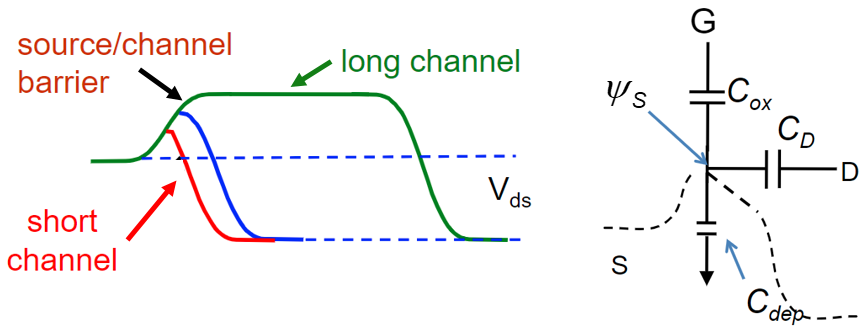
\includegraphics[width=0.8\textwidth]{figures/Fig5_2}
\centering
\caption{\small Illustration of channel potentials with various gate lengths and the equivalent circuit.}
\end{figure}
Similar to the concept in Chapter 1, the potential at the top-of-the-barrier can be written as \begin{equation}
    \psi_{S} = \frac{C_{OX}}{C_{OX}+C_{dep}+C_{D}}V_{GS} + \frac{C_{D}}{C_{OX}+C_{dep}+C_{D}}V_{DS}
\end{equation} where $C_{dep}$ is the depletion capacitance of the channel. From the Equation (5.47), $C_{D}$ gradually increase with shortening the gate length, and thus the drain voltage starts to control the barrier. If $V_{DS}$ is high, the threshould voltage ($V_{TH}$) is significantly degraded. This is called the {\bf drain-induced barrier lowering (DIBL)}. Furthermore, since the channel potential (charges) is controlled by (shared with) the drain terminal (even the source terminal), the threshold voltage is also decreasing even when $V_{DS}$ is low, which is known as {\bf $V_{TH}$ roll off}. The additional control from the drain terminal also deteriorates the subthreshold slope $SS$ \begin{equation}
    SS \equiv \left[\frac{\partial \log{I_{DS}}}{\partial V_{GS}}\right]^{-1} = 60\text{[mV/dec]}\times\left(1+\frac{C_{dep}+C_{D}}{C_{OX}}\right)
\end{equation} This is undesired since it significantly increases the OFF-state leakage current.
\subsubsection{Gate Tunneling Leakage}
Since the gate length is scaled to boost the current and allow more transistors in a give chip area, the gate oxide should be also scaled to improve the gate control as shown in the Equation (5.47). However, the thin oxide could lead to significant gate leakage due to the direct tunneling. Therefore, the high-$\kappa$ dielectric was introduced in the 45-nm technology node to keep the gate capacitance but increase the physical oxide thickness. Nevertheless, there are still some difficulties of the high-$\kappa$ dielectric: (1) chemical reactions between them and the silicon substrate and gate; (2) lower surface mobility than the Si/SiO$_{2}$ system; (3) too low a $V_{TH}$ for P-channel MOSFET (as if there is positive charge in the high-$\kappa$ dielectric); (4) long-term reliability; (5) a thin SiO$_{2}$ interfacial layer may be inserted between Si-substrate and high-$\kappa$ film.
\subsubsection{Mitigating Short Channel Effect of MOSFET}
Since the channel potential is also controlled by $C_{dep}$ and $C_{D}$, decreasing the depletion width by increasing the body doping is helpful but it may reduce the mobility due to the impurity scattering. Furthermore, using high-$\kappa$ metal gate as mentioned earlier also overcomes the poly-depletion problem. To cut the leakage path underneath the channel due to lack of gate control, the shallow junction is adopted. However, it enlarges the series resistance and thus degrades the ON-state current. To improve the mobility, strained silicon is used in the channel. In addition to the mentioned techniques to improve the device performances of the traditional MOSFET, new transistor structures [e.g. fully-depleted SOI (FDSOI) and FinFET] and new device operation mechanisms [e.g. tunnel FET (TFET) and negative capacitance FET (NCFET)] are proposed. The FDSOI can cut the leakage path and achieve low leakage, and the FinFET improves the gate control by increasing the gate capacitance. Furthermore, the TFET utilizes the tunneling mechanism which overcomes the problem from Boltzmann distribution, and the NCFET can achieve better subthreshold behavior since the channel potential can be boosted by the ferrroelctric layer sandwiched by the metal gate and interfacial layer.
\section{Application of the Developed Current Model}
The ballistic and quasi-ballistic current models have been derived. In this section, how the developed model relates to the real measurement data will be examined. Recall the Equation (5.47). At low $V_{GS}$ (let's say OFF-state), if the FDSOI or FinFET structure is adopted, the surface potential ($\psi_{S}$) in the channel is \begin{equation}
    \psi_{S} = \frac{C_{OX}}{C_{OX}+C_{D}}V_{GS} + \frac{C_{D}}{C_{OX}+C_{D}}V_{DS} \equiv \alpha_{G}V_{GS} + \alpha_{D}V_{DS}
\end{equation} where the contribution from the charge $Q$ is relatively small. The quasi-ballistic current is \begin{align}
    I^{OFF}& = (-e)W\frac{\sqrt{m_{x}m_{y}}k_{B}T}{2\pi\hbar^{2}}\sqrt{\frac{2k_{B}T}{\pi m_{x}}}e^{\frac{\mu_{S}}{k_{B}T}}e^{-\frac{E_{C}}{k_{B}T}}\left(1-e^{-\frac{eV_{DS}}{k_{B}T}}\right)/\left(1+\frac{2l_{eff}}{\lambda}\right),-E_{C}\rightarrow e\psi_{S}\nonumber\\
    & = (-e)W\frac{\sqrt{m_{x}m_{y}}k_{B}T}{2\pi\hbar^{2}}\sqrt{\frac{2k_{B}T}{\pi m_{x}}}e^{\frac{\mu_{S}}{k_{B}T}}e^{\frac{e\psi_{S}}{k_{B}T}}\left(1-e^{-\frac{eV_{DS}}{k_{B}T}}\right)/\left(1+\frac{2l_{eff}}{\lambda}\right)\nonumber\\
    & = Ae^{\frac{\alpha_{G}V_{GS}}{k_{B}T/e}}e^{\frac{\alpha_{D}V_{DS}}{k_{B}T/e}}\left(1-e^{-\frac{eV_{DS}}{k_{B}T}}\right) = Be^{\frac{\alpha_{G}V_{GS}}{k_{B}T/e}}
\end{align} Thus, the subthreshold slope is \begin{align}
    SS& = \left[\frac{\partial \log{I}}{\partial V_{GS}}\right]^{-1} = \frac{2.3k_{B}T/e}{\alpha} = 60/\alpha_{G}\text{[mV/dec]}\nonumber\\
    &= 60\times\left(1+\frac{C_{D}}{C_{OX}}\right)\text{[mV/dec]}\equiv 60\times m\text{[mV/dec]}
\end{align} where $m$ is called the body factor. The DIBL is defined as \begin{equation}
    \text{DIBL} = \frac{V_{TH}^{low}-V_{TH}^{high}}{V_{DS}^{high}-V_{DS}^{low}}\quad\text{[mV/V]}
\end{equation} where the threshold voltage $V_{TH}$ is defined using the constant current method \begin{equation}
    I_{TH} = Ae^{\frac{e\psi_{S}^{high}}{k_{B}T}} = Ae^{\frac{e\psi_{S}^{low}}{k_{B}T}}\frac{V_{DS}}{k_{B}T/e}
\end{equation} since \begin{equation}
    \left(1-e^{-\frac{eV_{DS}}{k_{B}T}}\right)\approx \frac{eV_{DS}}{k_{B}T},\quad\text{at low $V_{DS}$}\nonumber
\end{equation} where "low" and "high" denote as low and high $V_{DS}$, and \begin{equation}
    \psi_{S}^{low} = \alpha_{G}V_{TH}^{low} + \alpha_{D}V_{DS}^{low}
\end{equation} and \begin{equation}
    \psi_{S}^{high} = \alpha_{G}V_{TH}^{high} + \alpha_{D}V_{DS}^{high}
\end{equation} Thus, \begin{equation}
    \text{DIBL} = \frac{\alpha_{D}}{\alpha_{G}}-\frac{1}{\alpha_{G}}\frac{\psi_{S}^{high}-\psi_{S}^{low}}{V_{DS}^{high}-V_{DS}^{low}}
\end{equation} However, from the Equation (5.53) we have \begin{equation}
    \psi_{S}^{high}-\psi_{S}^{low} = \frac{k_{B}T}{e}\left[\ln{\frac{I_{TH}}{A}}-\ln{\frac{I_{TH}}{A}\frac{V_{DS}^{low}}{k_{B}T/e}}\right] = \frac{k_{B}T}{e}\ln{\frac{V_{DS}^{low}}{k_{B}T/e}}
\end{equation} which is very small since $V_{DS}^{low}$ is 50 mV\footnote{$V_{DS} =$ 50 mV is called the linear $V_{DS}$ and is commonly used. If applying $V_{DS} = $ 26 mV, the thermal noise could be an issue.}. Therefore, \begin{equation}
    \text{DIBL} = \frac{\alpha_{D}}{\alpha_{G}} = \frac{C_{D}}{C_{OX}}
\end{equation} which can be extracted from the subthreshold slope or the body factor.